% !TEX root = ../thesis.tex


\chapter{General Architecture}
\label{chap:gen_arch}
\label{sec:gen_arch}
Our reference architecture to deliver network services on the wide provider network is shown in Figure~\ref{fig:orchestrator}.
As evident from the picture, it allows the deployment of network services through three main portions, namely the \textit{service layer}, the \textit{orchestration layer} and the \textit{infrastructure layer}.

\begin{figure}[h]
	\centering
	% left bottom right top
	\includegraphics[clip= true, width= 1\columnwidth, trim= 0.5cm 0.5cm 1.7cm 0.0cm , page=4]{images/Pictures_definitivo.pdf}
	\caption{Overall view of the system.}
	\label{fig:orchestrator}
\end{figure}


\section{Service layer}
\label{sec:sl_intro}

The \textit{service layer} represents the external interface of our system and allows the different actors that can potentially use our solution (e.g., end users, the network provider, third-party organizations) to define their own network services. 

The input of this architectural part is hence a per-actor service description, expressed in an high level formalism  (called \textit{service graph} and detailed in Section~\ref{sec:service_graph}) capable of describing every type of service and also the potential interactions among different services. 
In order to facilitate the service creation, the actors should be provided with a graphical interface that makes available the components of the service (e.g., the VNFs), and which is integrated with an AppStore-like marketplace that enables the selection of a precise VNF among the many available.
The service graph should be provided together with several non-functional parameters. 
Particularly, we envision a set of \textit{Key Quality Indicators (KQIs)} specifying, for instance, the maximum latency allowed between two VNFs, or which is the maximum latency that can be introduced by the entire service. 
%The definition of the KQI may be implicitly done by the service layer logic, or could be left to the actors during the definition of their services.
We also foresee the definition of a list of high-level policies to be taken into account during the deployment of the service.
An example of such policies could be the requirement of deploying the service in a specific country because of legal reasons.

Given the above inputs, the service layer should be able to translate the service graph specification into an orchestration-oriented formalism, namely the \textit{forwarding graph} detailed in Section~\ref{sec:forwarding_graph}. 
This new representation provides a more precise view of the service to be deployed, both in terms of computing and network resources, namely Virtual Network Functions (VNFs) and interconnections among them, always conserving KQIs and policies imposed by the actor who defined the service.

The service layer should also define some APIs to be exported to the lower layers of the architecture, so that it can be notified of some low level events that could be exploited to implement the service logic. 
An example of such events may be the connection of a terminal device (e.g., a laptop) to the network, which could trigger the deployment of a new service graph in the service layer.

% Architecture and design principle
As depicted in Figure~\ref{fig:orchestrator}, the service layer includes a component implementing the service logic (identified with the service layer application (SLApp) block in the picture), in addition to an interface that can be called when specific events occur (e.g., a new end user attaches to the network) and that triggers the deployment/update of a service graph. This logic (and the corresponding implementation) is strictly related to the use case under consideration. 
Particularly, in this thesis we consider the case in which the \textit{end users} connected to the network, as well as the \textit{Internet Service Provider (ISP)}, can provide a description of services to be implemented in network of the ISP itself.

However, it is worth pointing out that the service northbound interface design principles are very similar to a generic public-cloud API, such as Amazon Web Services (AWS)~\cite{aws}. 
In fact, the service layer could not only be used to conceive services in a typical ISP provider-customer scenario, but it opens the door to third-party providers to be involved into custom-service definition. 
In effect, this interface enables a cloud-like service delivering in which 3rd-party providers (e.g., content-providers) could offer services on an ISP infrastructure, orchestrating resources on demand and being billed for their utilization in a pay-per-use fashion. 
%FABIO: In that way?? 


\section{Orchestration layer}
\label{sec:general_orch}
The orchestration layer sits below the service layer, and it is responsible of two important phases in the deployment of a service on the physical infrastructure.
First, it manipulates the forwarding graph in order to allow its deployment on the infrastructure; these transformations include the enriching of the initial definition with extra-details such as new VNFs, as well as the consolidation of several VNFs into a single one. Second, the orchestration layer implements the scheduler that is in charge of deciding where to instantiate the requested service. The scheduling could be based on different classes of parameters: (i) information describing the VNF, such as the CPU and the memrory required; (ii) high-level policies and KQIs provided with the forwarding graph; (iii) resources available on the physical infrastructure, such as the presence of a specific hardware accelerator on a certain node, as well as the current load of the nodes themselves.

% Architecture and design principle
As depicted in Figure~\ref{fig:orchestrator}, the orchestration layer is composed of three different logical sub-layers. 

First, the \textit{orchestration} sub-layer implements the orchestration logic (forwarding graph transformation and scheduling) in a technology-independent approach, without dealing with details related to the infrastructure implementation. 
The next component, called \textit{controller adaptation} sub-layer, implements instead the technology-dependent logic that is in charge of translating the (standard) forwarding graph into the proper set of calls for the northbound API of the different infrastructure controllers.
These controllers correspond to the bottom part of the orchestration layer, and are in charge of applying the above commands to the resources available on the physical network; the set of commands needed to actually deploy a service is called \textit{infrastructure graph} (Section~\ref{sec:ig}), and changes according to the resource on which the service is going to be instantiated.
In practice, the infrastructure controllers transform the forwarding graph into the proper set of calls for the northbound API of the different infrastructure controllers, to be executed on the physical infrastructure in order to deploy the service.
The infrastructure controllers should also be able to identify the occurrence of some events in the infrastructure layer (e.g., a new flow from an unknown device arrives to one node), and to notify it to the upper layers of the architecture.

As shown in Figure~\ref{fig:orchestrator}, different kind of nodes require different implementations for the infrastructure controllers (in fact, each type of nodes has its own controller), which in turn require many \textit{control adapters} in the controller adaptation sub-layer.
Moreover, the orchestration sub-layer and the controller adaptation sub-layer are merged together into the \textit{global orchestrator} module.

Having in mind the heterogeneity (e.g., core and edge technologies) and size of the provider network, it is quite evident how the orchestration layer (and in particular the global orchestrator, which sits on top of many resources) is critical in terms of performance and scalability %and resilience 
of the entire system. 
For this reason, according to the picture, the global orchestrator has syntactically identical northbound and southbound interfaces (in fact, it receives a forwarding graph from the service layer, and it is able to provide a forwarding graph to the next component), which opens the door to a hierarchy of orchestrators %is possible 
in our architecture.
This would enable the deployment of a forwarding graph across multiple administrative domains in which the lower level orchestrators expose only some information to the upper level counterparts, so that %which allows 
the architecture can scale up with a huge number of physical resources in the infrastructure layer.
Although such a hierarchical orchestration layer is an important aspect of our architecture, it is out of the scope of this thesis and it is not considered in the implementation detailed in Section~\ref{sec:global_orch}.

%This component can include an infrastructure-dependent scheduler, which determines the best location of the requested resources (e.g., VMs) based on infrastructure-related parameters. For example, given a VM implementing a specific network function, this scheduler is in charge of selecting the best server that is compatible with the VM image (e.g., in terms of hypervisor, CPU architecture, etc) and that has enough resources to run that service.

\section{Infrastructure layer}

The \textit{infrastructure layer} sits below the orchestration layer and includes the physical resources where the required service is actually deployed.
From the point of view of the orchestration layer, it is organized in nodes, each one having its own infrastructure controller; the global orchestrator can potentially schedule the forwarding graph on each one of these nodes.
Given the heterogeneity of modern networks, we envision the possibility of having multiple nodes implemented with different technologies; in particular, we consider two classes of infrastructure resources.

The first class consists in cloud-computing domains, and it is called \textit{OpenStack-based node} in Figure~\ref{fig:orchestrator}, referencing one of most popular cloud management toolkit (Chapter~\ref{chap:Utilized Tools}).  
Each OpenStack-based node actually consists of a cluster of physical machines managed by the same infrastructure controller.

The second class of resources is instead completely detached by traditional cloud-computing environments. 
In fact, we envision that some useful resources to execute VNFs could be outside of the datacenter, such as the 
traditional (or improved) home-gateways hosted in the end users' homes. 
An element of this class, shown in the bottom-right part of Figure~\ref{fig:orchestrator} and called \textit{integrated node}, consists of a single physical machine and it is mostly based on dedicated software.
Note that, in this case, the infrastructure controller is integrated in the same machine hosting the required service.

As a final remark, the infrastructure layer does not implement any logic (e.g., packet forwarding, packet processing) by itself; in fact, it is completely configurable, and each operation must be defined with the deployment of the proper forwarding graph.
This makes our architecture extremely flexible, since it is able to implement each type of service and use case defined in the service layer.

%belonging to the same data center\footnote{As described later, the FG can be split so that different parts are deployed on different physical servers, according to the resources available on the machines.}.
%For instance, Figure~\ref{fig:orchestrator} shows how we foreseen two different implementations for this layer, which are needed to accommodate the objectives listed in Section~\ref{sec:intro}.
%In the first implementation, depicted in the bottom-left part of the picture, 
%As evident from the figure, in this case the network/compute/storage layer consists of some OpenStack components, which takes care of deploying the FG on the proper servers.
